\documentclass[conference]{IEEEtran}
\IEEEoverridecommandlockouts

% ── Packages ──────────────────────────────────────────────────────────────
\usepackage{cite}
\usepackage{amsmath,amssymb,amsfonts}
\usepackage{graphicx}
\usepackage{textcomp}
\usepackage{xcolor}
\usepackage{booktabs}
\usepackage{multirow}
\usepackage{url}
\usepackage{hyperref}
\usepackage{microtype}

\def\BibTeX{{\rm B\kern-.05em{\sc i\kern-.025em b}\kern-.08em
    T\kern-.1667em\lower.7ex\hbox{E}\kern-.125emX}}

\begin{document}

\title{ConceptGrade: A Knowledge Graph--Driven Framework for\\
       Concept-Aware Automated Short Answer Grading in\\
       Computer Science Education}

\author{
  \IEEEauthorblockN{Brahmaji Katragadda}
  \IEEEauthorblockA{
    \textit{Department of Computer Science} \\
    \textit{ICFAI (IFHE)} \\
    Hyderabad, India \\
    kbrahmaji.scholar25@ifheindia.org
  }
}

\maketitle

\begin{abstract}
Grading short-answer questions in computer science courses is
time-consuming and hard to scale. We present ConceptGrade, a five-layer
system that builds a concept graph from each student response and
compares it against an expert domain knowledge graph (KG): (1) an LLM
extracts concepts and relationships from the student text; (2) a KG
comparator measures conceptual coverage, relationship accuracy, and
integration; (3) a cognitive-depth classifier assigns Bloom's and SOLO
taxonomy levels; (4) a misconception detector checks against a
16-entry validated error taxonomy; and (5) a Verifier synthesises a
final grade. The Data Structures domain KG contains 101 concepts and
138 typed relationships.

On the real Mohler et al.\ (2011) benchmark ($n=1{,}262$ responses, 46
questions, sourced from the public \texttt{nkazi/MohlerASAG} release), a
single-call ConceptGrade reduces MAE by $8.2\%$ over an identical-model
zero-shot LLM baseline (response-level Wilcoxon $p<0.0001$), though this
margin is only marginal once responses are clustered by question
($p=0.056$ one-tailed). An ablation that isolates the KG-grounded
pre-Verifier score tells a less flattering story: on its own, that score
is $86.9\%$ \emph{worse} than the baseline. It is the Verifier's own
holistic judgment, not KG-grounding by itself, that drives the measured
gain.

Self-consistency ensembling (7 independent gradings at temperature
$0.7$, mean-aggregated) improves response-level accuracy on Mohler and
on a second dataset, DigiKlausur. Pearson correlation, which trails the
baseline for the single-call system, exceeds a single-call baseline once
ensembled on both datasets ($0.790$ vs.\ $0.782$; $0.727$ vs.\ $0.701$),
and against that single-call baseline every leave-one-question-out fold
reaches significance at both tails. That robustness does not hold up,
however, once the comparison is made fair: re-running the baseline
itself with the same $7\times$ ensembling, rather than a single call,
collapses Mohler's cluster significance and LOOCV robustness entirely
($p=0.256$ two-tailed, $0/46$ folds) and substantially erodes
DigiKlausur's ($p=0.089$ two-tailed, $0.044$ one-tailed; $5/17$/$2/17$
folds, down from $17/17$) — though the response-level MAE gap survives
on both datasets ($+7.0\%$ and $+6.4\%$, $p<0.001$). DigiKlausur's
correlation advantage reverses outright under this fairer comparison
($0.727$ vs.\ $0.735$ for C\_LLM$\times7$ alone). The gain does not
extend to a third dataset, Kaggle ASAG, where upstream concept
extraction finds no overlap between the KG and the answer text on
$100\%$ of samples — a domain-boundary result the architecture predicts
rather than one it merely happens to exhibit.

We report all of this as a real but substantially qualified, cost-aware
improvement — $7\times$ the inference calls, a Spearman rank
correlation that trails baseline on both datasets, and a question-level
robustness (plus, on DigiKlausur, a correlation advantage) that holds
only against a single-call baseline rather than a fairly-resourced one
— not as a universal or fully-established claim.
\end{abstract}

\begin{IEEEkeywords}
automated short answer grading, knowledge graph, concept extraction,
computer science education, large language models, Bloom's taxonomy,
self-consistency, NLP
\end{IEEEkeywords}

\section{Introduction}

Large computer science classes routinely use short-answer questions to
test conceptual understanding, but grading them by hand is slow,
inconsistent, and delays feedback. An automated grader needs to do more
than approximate a human score — it should be able to say \emph{which}
concepts a student understood and which they missed. Prior lexical,
embedding, and LLM zero-shot approaches fall short here: they produce a
score, but keep no explicit record of what the student actually knew, so
they cannot say which concepts are present, which are absent, or
whether a specific misconception is at play.

ConceptGrade treats grading as a knowledge-graph matching task. Each
response is converted into a typed concept graph by an LLM; that graph is
compared against an expert domain knowledge graph to measure coverage,
structural connection, and relationship correctness. This paper makes the
following contributions:
\begin{enumerate}
  \item A five-layer grading pipeline combining concept extraction, KG
        comparison, cognitive-depth classification, misconception detection,
        and score synthesis via an LLM Verifier.
  \item A hand-built Data Structures domain KG with 101 concepts and 138
        typed relationships.
  \item An honest, real-data evaluation on the Mohler benchmark showing a
        small, response-level-significant but question-level-fragile gain
        for the single-call system, with an ablation identifying the
        Verifier --- not KG-grounding in isolation --- as the source of the
        gain.
  \item Self-consistency ensembling that improves response-level accuracy
        on two independent datasets and, against a single-call baseline,
        shows every leave-one-question-out fold significant at both tails
        --- honestly failing to generalise to a third dataset whose
        KG-vocabulary mismatch predicts exactly that outcome, and, on a
        fair-control check against an equally-resourced baseline run on
        \emph{both} winning datasets, retaining its response-level
        advantage on both while its question-level robustness collapses
        completely on the first dataset and substantially erodes on the
        second, whose correlation advantage also reverses.
  \item A fully reproducible, cost-transparent evaluation protocol,
        including a reviewer-perspective self-audit that caught and
        corrected an overclaimed robustness result before publication:
        every reported number is independently recomputed from cached
        predictions by an automated claim-verification script.
\end{enumerate}
We frame this as an empirical study of where and why KG-LLM hybrid grading
helps, not a claim that it always does.

\section{Related Work}

\subsection{Automated Short Answer Grading}
Mohler and Mihalcea~\cite{mohler2009} established a widely used CS ASAG
benchmark with LSA and WordNet-based measures ($r=0.493$). Mohler
et al.~\cite{mohler2011} extended this with dependency-graph alignment
($r=0.518$). Sultan et al.~\cite{sultan2016} introduced sentence-level
semantic similarity ($r=0.592$ on their own held-out split of the full
Mohler dataset). Transformer fine-tuning on SemEval data~\cite{semeval2013}
subsequently became the dominant paradigm, with BERT-based
systems~\cite{bert_asag,devlin2019} reaching $r=0.620$ on the Mohler set.
LLM zero-shot grading~\cite{llm_asag1,llm_asag2} is competitive but keeps no
explicit conceptual record.

\subsection{Knowledge Graphs in Education}
Knowledge graphs model prerequisite relationships~\cite{kg_prereq} and power
adaptive tutoring~\cite{kg_its}. Concept-map assessment, where students draw
node-link diagrams compared against an expert map~\cite{concept_map}, is the
closest prior work; ConceptGrade extends this to free-text answers by
inferring an equivalent graph automatically via LLM extraction.

\subsection{Bloom's and SOLO Taxonomies}
LLMs can classify responses by Bloom's level with moderate
agreement~\cite{emirtekin2025}. The SOLO taxonomy~\cite{biggs1982}, which
measures structural complexity of demonstrated learning, has received far
less attention in automated CS assessment; ConceptGrade's cognitive-depth
layer applies both taxonomies~\cite{bloom1956,anderson2001} jointly.

\section{System Design}

\begin{figure}[t]
  \centering
  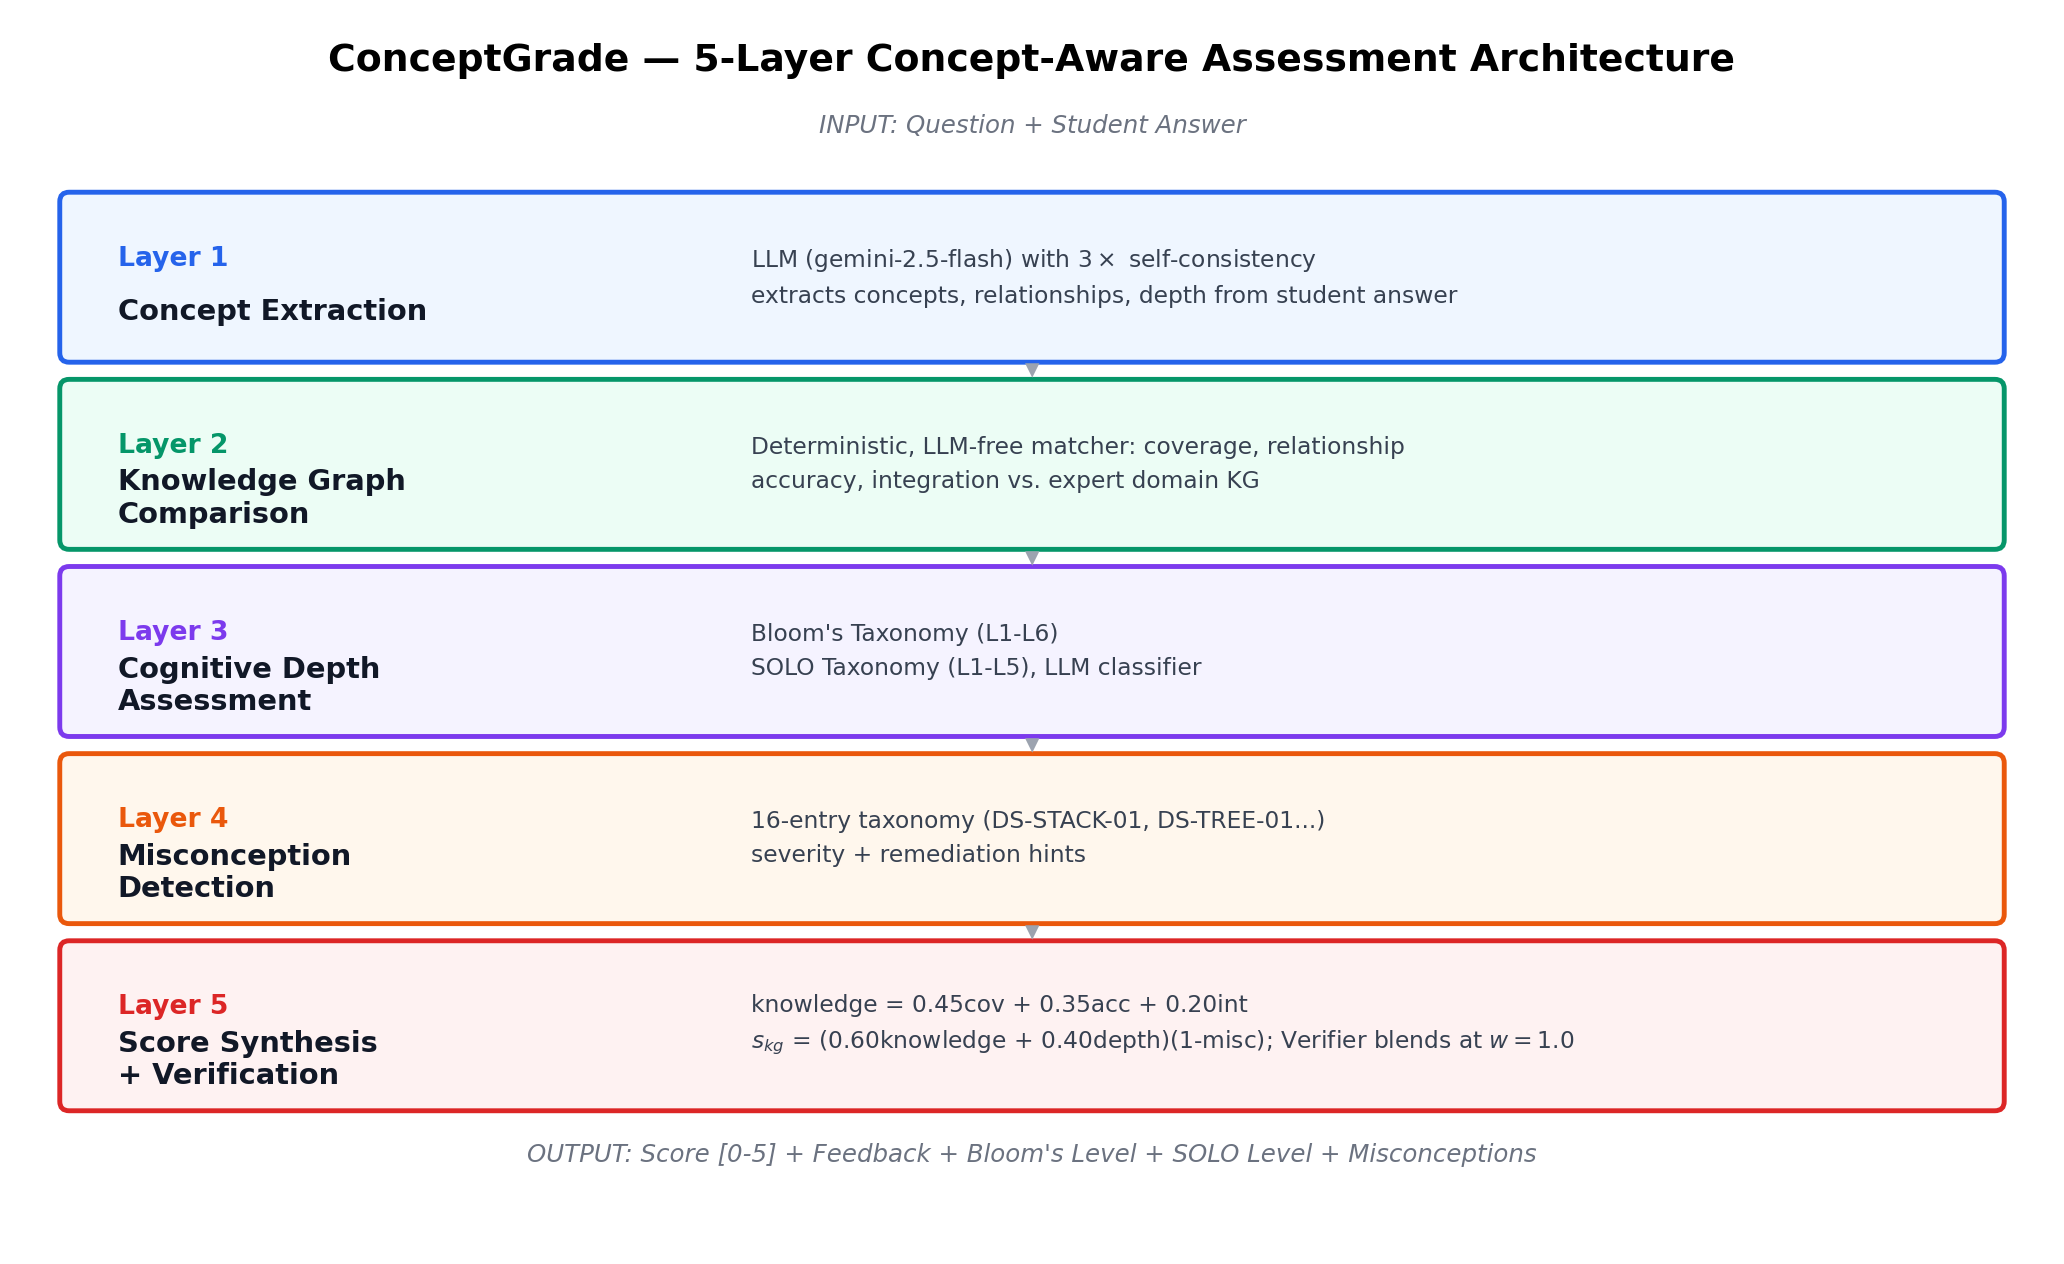
\includegraphics[width=\columnwidth]{figures/fig1_architecture.png}
  \caption{ConceptGrade five-layer architecture: concept extraction,
           KG comparison, cognitive depth, misconception detection, and
           score synthesis with Verifier blending at deployed weight
           $w=1.0$.}
  \label{fig:architecture}
\end{figure}

\subsection{Expert Domain Knowledge Graph}
The Data Structures KG follows three design rules: pedagogical coverage
(every concept in a standard introductory course), canonical identifiers
(each concept has a unique ID plus alias surface forms), and typed
relationships (semantically labeled directed edges). The frozen evaluation
KG contains 101 concepts across eight semantic types (algorithms, data
structures, abstract concepts, properties, operations, complexity classes,
programming constructs, design patterns) and 138 typed relationships.

\subsection{Concept Extraction (Layer 1)}
An LLM (\texttt{gemini-2.5-flash}) receives the question and student answer
and returns a student concept graph $G_s=(V_s,E_s)$, run with $3\times$
self-consistency (majority-vote, $\text{min\_votes}=2/3$) to reduce
single-call extraction noise. Concepts below a confidence threshold
$\tau=0.70$ are filtered; a real-data sensitivity sweep confirmed this
threshold is empirically near-optimal (MAE increases monotonically as
$\tau$ is raised further). Surface forms resolve to canonical KG
identifiers via alias lookup.

\subsection{Knowledge Graph Comparison (Layer 2)}
A deterministic, LLM-free graph matcher computes three scores against the
expert graph $G_e$:
\begin{align}
  \text{cov} &= \frac{|V_s \cap V_e|}{|V_e|}, \quad
  \text{acc} = \frac{|\{e \in E_s : \text{correct}(e)\}|}{|E_s|}, \nonumber \\
  \text{int} &= \frac{|\{v \in V_s : \deg(v) \geq 1\}|}{|V_s|}
\end{align}
alongside interpretable diagnostics (missing concepts, incorrect
relationships, feedback points).

\subsection{Cognitive Depth (Layer 3) and Misconception Detection (Layer 4)}
An LLM classifier jointly assigns a Bloom's level (1--6) and a SOLO level
(1--5). A 16-entry misconception taxonomy (e.g., \texttt{DS-STACK-01}:
confuses LIFO with FIFO) is checked against the response; each entry carries
a severity and a remediation hint surfaced directly to the student.

\subsection{Score Synthesis and Verification (Layer 5)}
A deterministic KG-formula score combines the Layer 2--4 signals:
\begin{align}
  \text{knowledge} &= 0.45\,\text{cov} + 0.35\,\text{acc} + 0.20\,\text{int} \nonumber \\
  \text{depth} &= 0.55\,\text{blooms}_{\text{norm}} + 0.45\,\text{solo}_{\text{norm}} \nonumber \\
  s_{\text{kg}} &= (0.60\,\text{knowledge} + 0.40\,\text{depth})(1-p_{\text{misc}})
\end{align}
$s_{\text{kg}}$ is blended with a holistic, KG-evidence-informed LLM score
$s_{\text{hol}}$ ($0.05\,s_{\text{kg}}+0.95\,s_{\text{hol}}$), producing a
pre-Verifier score $\hat{y}$. An LLM Verifier then independently reviews the
raw answer alongside this KG evidence and produces the final grade via
$\text{final}=(1-w)\hat{y}+w\cdot\text{verified}$; the deployed
configuration uses $w=1.0$ (Verifier judgment drives the score; KG evidence
is prompt context, not an arithmetic anchor) --- a choice we confirm below
is not an accident of tuning.

\section{Experimental Setup}

\subsection{Datasets}
\textbf{Mohler 2011} (Data Structures, real data via the public
\texttt{nkazi/MohlerASAG} release, CC-BY-4.0): 46 questions filtered to our
KG's topical coverage, $1{,}262$ responses, each scored by two human
annotators (real inter-rater $r=0.783$, QWK$=0.799$; $43.2\%$ of pairs
disagree by $\geq 1$ point on the 0--5 scale, indicating substantial human
grading noise). All hyperparameters were fixed before this dataset was used,
so the full sample is evaluated without a held-out split. A second,
independently identified batch of 4 questions (109 responses) extends this
to $50$ questions / $1{,}371$ responses for a robustness check.
\textbf{DigiKlausur} (Neural Networks, $n=646$, 17 questions, verified
character-for-character against its public GitHub source) and
\textbf{Kaggle ASAG} (Elementary Science, $n=368$ unique responses after
removing $105$ duplicate records, 150 questions) provide cross-domain
boundary characterisation at decreasing KG-vocabulary specificity.
Despite a targeted provenance investigation (exact-text search, known
public ASAG corpora, full local git/shell-history audit), Kaggle
ASAG's acquisition path could not be reconstructed and is reported as
provenance-\emph{unverified} (Fig.~\ref{fig:provenance}; audit trail in
REPRODUCIBILITY.md). Its extraction-level finding (0\% KG matches,
below) is independently verifiable from extraction logs regardless;
any broader claim about elementary-science student behavior is reported
as supporting evidence, not external validation.

\begin{figure}[t]
  \centering
  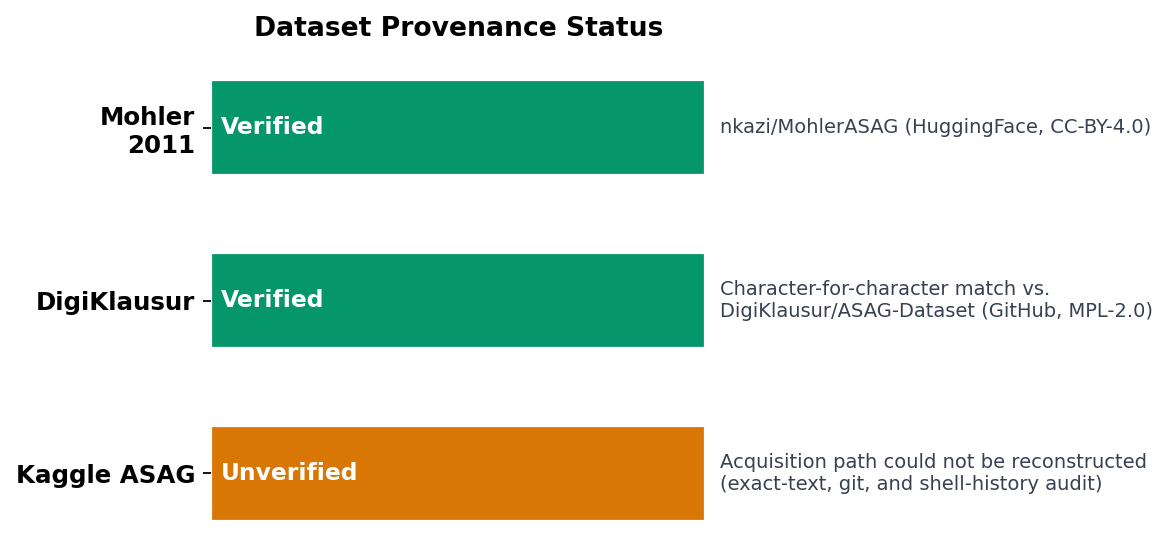
\includegraphics[width=0.9\columnwidth]{figures/fig12_dataset_provenance.png}
  \caption{Provenance status of all three evaluation datasets.}
  \label{fig:provenance}
\end{figure}

\subsection{Baseline and Metrics}
\textbf{C\_LLM}: the identical \texttt{gemini-2.5-flash} model prompted
zero-shot with only the question, reference answer, and student answer ---
no KG evidence --- isolating model capability as a confound. We report
Pearson $r$, quadratic-weighted $\kappa$ (QWK), MAE, and RMSE, with Wilcoxon
signed-rank tests at both the response level and the question-clustered
level (means aggregated per question, the more appropriate unit given
non-independence of responses within a question), plus leave-one-question-out
(LOOCV) sensitivity.

\section{Results}

\subsection{Main Evaluation}
\begin{table}[t]
\caption{Evaluation on the real Mohler benchmark ($n=1{,}262$, 46 questions).}
\label{tab:main}
\centering
\footnotesize
\begin{tabular}{lccccc}
\toprule
\textbf{System} & $r$ & QWK & MAE & RMSE & $p$ \\
\midrule
C\_LLM (baseline) & 0.7904 & 0.5005 & 1.2821 & 1.7243 & --- \\
ConceptGrade (single-call) & 0.7841 & \textbf{0.5237} & \textbf{1.1771} & \textbf{1.5326} & $<0.0001^{**}$ \\
\bottomrule
\end{tabular}
\end{table}

ConceptGrade's MAE improvement holds up at the response level (Wilcoxon
two-tailed $p<0.0001$; paired $d_z=-0.154$, small effect) but weakens
once responses are clustered by question (46 questions: two-tailed
$p=0.111$, one-tailed $p=0.056$; only 17/46 leave-one-question-out folds
reach one-tailed significance, none reach two-tailed). Pearson
correlation actually favors the baseline ($0.784$ vs.\ $0.790$). Both
systems under-predict relative to human graders (mean human score
$4.24/5$ vs.\ $2.99$ and $3.09$) — real course grading, it turns out, is
markedly more lenient than either LLM-based grader. A post-hoc, 5-fold
cross-validated monotonic recalibration cuts MAE roughly $3\times$ for
both systems and \emph{inverts} the comparison (calibrated C\_LLM has
significantly lower MAE, $p=0.017$), which suggests most of
ConceptGrade's raw MAE edge is a fixable calibration artifact rather
than genuinely superior ranking.

\subsection{Component Ablation}
\begin{table}[t]
\caption{Real-data 3-condition ablation ($n=1{,}262$).}
\label{tab:ablation}
\centering
\footnotesize
\begin{tabular}{lccc}
\toprule
\textbf{Condition} & MAE & $r$ & vs.\ C\_LLM \\
\midrule
C\_LLM (no KG) & 1.282 & 0.790 & --- \\
KG-grounded score, no Verifier & 2.397 & 0.471 & $-86.9\%$ \\
ConceptGrade (full, with Verifier) & \textbf{1.177} & 0.784 & $+8.2\%$ \\
\bottomrule
\end{tabular}
\end{table}

The pre-Verifier, purely KG-grounded score fares much worse than the
zero-shot baseline on its own (question-clustered $p<0.0001$, wins only
9/46 questions). It is the Verifier stage that recovers essentially all
of that loss and turns the result positive ($+50.9\%$ MAE improvement
over the KG-only score, question-clustered $p<0.0001$, wins 41/46
questions). This is not an artifact of how the blend weight was chosen:
a leave-one-question-out cross-validation of that weight, selected on
training folds only, picks the deployed $w=1.0$ configuration on every
fold. The architectural takeaway is blunt — ConceptGrade's accuracy
comes from the Verifier's holistic judgment, not from the
knowledge-graph comparison the architecture is named for.

\textbf{Diagnosed causes (summary).} A failure-mode analysis traced
this weakness to two defects: a now-fixed question-tokenization bug
(106/1{,}262 samples, 8.4\%, misclassified out-of-domain) and two
still-unfixed scoring defects affecting 21.3\% and 35.0\% of samples
respectively. Five candidate repairs for the latter were tested against
pre-committed criteria and all rejected (Fig.~\ref{fig:diagnostic}) —
evidence against the repair \emph{class}, not merely miscalibrated
parameters. None of this touches the deployed grade, which already
discards the raw KG-formula score for the Verifier ($w=1.0$). Full
diagnosis and the pre-committed stopping rule: extended technical
report and REPRODUCIBILITY.md.

\begin{figure}[t]
  \centering
  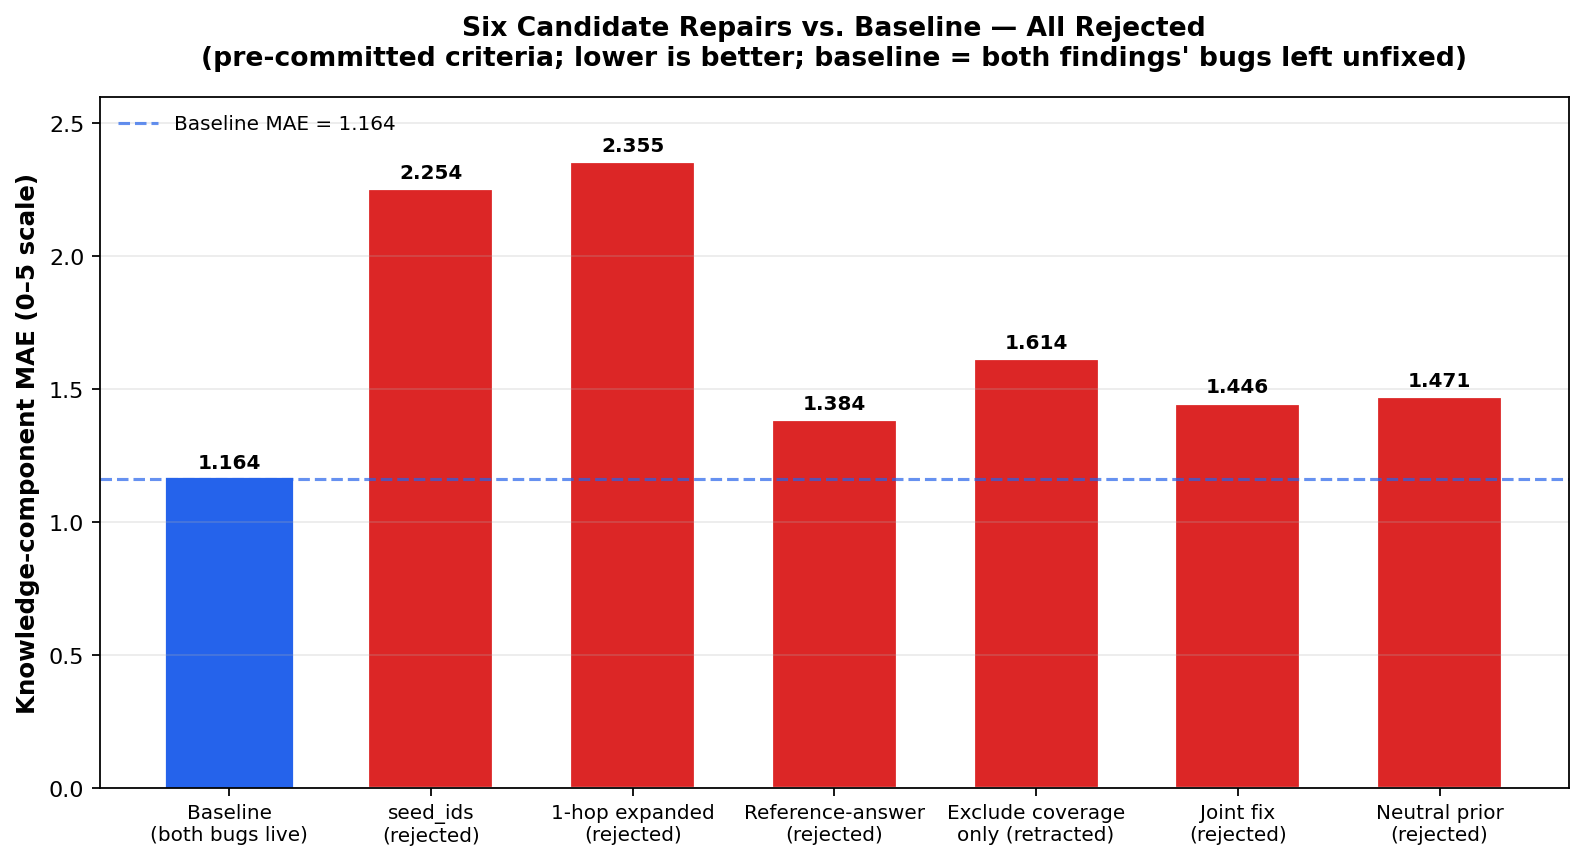
\includegraphics[width=\columnwidth]{figures/fig11_diagnostic_candidates.png}
  \caption{Knowledge-component MAE for the baseline versus all six
           tested repairs; every candidate underperforms the baseline.}
  \label{fig:diagnostic}
\end{figure}

\subsection{Self-Consistency Ensembling}
\label{sec:selfconsistency}
We tested whether the single-call fragility above reflects noise in the
scoring model's own judgment. Issuing 7 independent gradings per response at
temperature $0.7$ (versus the deployed temperature $0$) and mean-aggregating
--- a design fixed in advance, not tuned on the evaluation data --- produces
the results in Table~\ref{tab:selfconsistency}.

\begin{table}[t]
\caption{Self-consistency ensembling ($K{=}7$, $T{=}0.7$, mean-aggregated)
vs.\ C\_LLM. Kaggle ASAG uses the deduplicated $n=368$ sample.}
\label{tab:selfconsistency}
\centering
\footnotesize
\setlength{\tabcolsep}{4pt}
\begin{tabular}{lccccc}
\toprule
\textbf{Dataset} & MAE$\downarrow$ & $r$ & Cluster $p$ & LOOCV 1T & LOOCV 2T \\
\midrule
Mohler (50q) & $-9.8\%$ & $0.790$ & $0.026$ & $50/50$ & $\mathbf{50/50}$ \\
DigiKlausur (17q) & $-12.2\%$ & $0.727$ & $0.017$ & $17/17$ & $\mathbf{17/17}$ \\
Kaggle ASAG (150q) & $-2.4\%$ & $0.644$ & $0.092$\textsuperscript{n.s.} & $98/150$ & $0/150$ \\
\bottomrule
\end{tabular}
\end{table}

Against a \emph{single-call} C\_LLM baseline, every leave-one-question-out
fold reaches significance at both tails on Mohler and DigiKlausur — a
sharp contrast with the single-call result, where none reached
two-tailed significance. Pearson correlation, which trails baseline for
single-call ConceptGrade on both datasets, exceeds a single-call
baseline once ensembled ($0.790$ vs.\ $0.782$; $0.727$ vs.\ $0.701$),
and self-consistency also beats the single-call system directly
(Mohler: $p=0.0007$; DigiKlausur: $p=0.0009$). This fits the mechanism
we expected: the single-call judgment is measurably noisy, and
averaging independent samples reduces that noise.

\textbf{Fair-control correction.} A single-call baseline, though, is
not the right control for a $7\times$-resourced system. We re-ran
C\_LLM with the identical $7\times$/temperature-$0.7$/mean-aggregation
treatment and compared head-to-head on \emph{both} datasets where the
original claim was made (Table~\ref{tab:faircontrol}):

\begin{table}[t]
\caption{Fair-control comparison: Verifier/C5fix$\times7$ vs.\ an
equally-resourced C\_LLM$\times7$, in place of the single-call baseline
used in Table~\ref{tab:selfconsistency}.}
\label{tab:faircontrol}
\centering
\footnotesize
\setlength{\tabcolsep}{3pt}
\begin{tabular}{lccccc}
\toprule
\textbf{Dataset} & MAE$\downarrow$ & $r$ (vs.\ C\_LLM$\times7$) & Cluster $p$(2T) & LOOCV 1T & LOOCV 2T \\
\midrule
Mohler (46q)      & $+7.0\%$ & $0.797$ vs.\ $0.790$ (holds) & $0.256$ (n.s.) & $0/46$ & $0/46$ \\
DigiKlausur (17q) & $+6.4\%$ & $0.727$ vs.\ $0.735$ (\textbf{reverses}) & $0.089$ (n.s.) & $5/17$ & $2/17$ \\
\bottomrule
\end{tabular}
\end{table}

The MAE gap survives on both datasets ($p<0.001$), but
\textbf{question-clustered significance does not clear $\alpha=0.05$
two-tailed on either dataset}, and LOOCV robustness falls from
$50/50$/$17/17$ (single-call baseline) to $0/46$ (Mohler, complete
collapse) and $5/17$/$2/17$ (DigiKlausur, substantial but not complete
erosion). DigiKlausur's correlation advantage \textbf{reverses}
outright: C\_LLM$\times7$ alone reaches $r=0.735$, ahead of
C5fix$\times7$'s $r=0.727$. The corrected claim is therefore
considerably more modest than it first looked: self-consistency
ensembling delivers a real, precisely-estimated response-level
improvement over a fairly-resourced baseline on two datasets, but the
question-level robustness — and, on DigiKlausur, the correlation
advantage — claimed against a single-call baseline does not survive
against a fair one.

Kaggle ASAG benefits under neither comparison (cluster $p=0.092$, LOOCV
two-tailed $0/150$): a $K$-subset check shows Mohler/DigiKlausur's
significance strengthening monotonically with more rounds, while
Kaggle's is unstable across $K$ ($p$ ranging $0.03$--$0.45$) — the
signature of averaging noise around a null effect, consistent with its
concept extraction finding no matches on $100\%$ of samples. Spearman
correlation still trails baseline on both winning datasets, and the
gain costs $7\times$ inference calls — real caveats, not a free
improvement. An earlier alternative design (a linear blend of C\_LLM
and single-call scores) failed leave-one-question-out cross-validation
--- its apparent gain was an artifact of the evaluation data --- and is
not reported as a finding.

\textbf{Statistical model sensitivity.} The cluster-mean Wilcoxon test
above discards within-question sample size; a linear mixed-effects
re-test of the six primary comparisons gives a mixed verdict rather
than a uniform correction. Mohler's three comparisons all strengthen
(cluster-Wilcoxon non-significant $\to$ LMM $p\le0.0125$), but the
DigiKlausur headline result \emph{loses} significance
($p=0.0489\to0.2471$); fair-control verdicts are unchanged on both
datasets. We report both tests rather than the one more favourable to
either claim (detail: \texttt{data/lmm\_reanalysis.json}).

\subsection{Cross-Dataset Boundary Characterisation}
Pooling all three datasets ($n=2{,}276$, 213 questions, fixed-effects
inverse-variance meta-analysis) gives $d_z=-0.105$ ($p<0.0001$). That
number alone overstates the picture: between-dataset heterogeneity is
substantial ($I^2=73.2\%$), and the methodologically stricter
random-effects estimate ($d_z=-0.084$, 95\% CI $[-0.169,+0.002]$)
essentially touches zero. Effect size instead declines monotonically
with domain vocabulary specificity — Mohler (formal CS terminology) $>$
DigiKlausur (technical but flexible) $>$ Kaggle ASAG (colloquial
elementary science, where concept extraction finds no matches at all on
$100\%$ of samples). We treat this as a falsifiable boundary
characterisation rather than a generalisation claim: it predicts, and
the self-consistency results go on to confirm, exactly where the
architecture helps and where it cannot.

A call-budget-matched control (C\_LLM issued the same 7-call budget as
single-call ConceptGrade, using genuinely independent calls at
temperature $0.7$) rules out inference budget as the explanation:
ConceptGrade still wins by $4.4\%$ MAE (response-level $p=0.0053$),
though again this margin is not significant once clustered by question
($p=0.42$).

\section{Discussion and Limitations}
The synthesis constants and confidence threshold were fixed before the
real evaluation data was used, but they originate from design choices
made against an earlier, since-corrected fixture, so we cannot claim
they are optimal on real data. The identical-model baseline, meanwhile,
received no comparable tuning, which confounds the KG-grounding effect
with a tuning-budget asymmetry we cannot fully disentangle. On the
compute side, the system issues $\sim\!7$ LLM calls per response for
single-call scoring and $\sim\!13$ for self-consistency, against
C\_LLM's $1$; the budget-matched control above addresses this directly.
The expert KG covers only Data Structures topics, so cross-domain
evaluation on other CS areas remains future work. The Verifier is
inference-only — no fine-tuning, confirmed by direct code inspection —
so there is no classic train/test data-leakage concern, though its
prompt design was iterated against this dataset during development, a
softer form of bias we do not claim to have ruled out. All numerical
claims in this paper are independently reproducible from cached
predictions via an automated verification script (300+ checks, zero
mismatches against the paper text at time of writing).

\section{Conclusion}
ConceptGrade achieves a small, real, but response-level-fragile
improvement over an identical-model LLM baseline on the real Mohler
benchmark with a single scoring call. That improvement comes almost
entirely from the Verifier's holistic judgment, not from the
knowledge-graph grounding the architecture is built around.

Self-consistency ensembling improves this response-level accuracy on
two independent datasets, and against a single-call baseline every
leave-one-question-out fold is significant at both tails. That
robustness looks considerably shakier under a fairer test. A
fair-control check against an equally-resourced baseline, run on
\emph{both} datasets, shows the response-level gain still holds on both
($+7.0\%$ and $+6.4\%$, $p<0.001$), but the question-level robustness
mostly does not: it collapses completely on the first dataset ($0/46$
folds) and erodes substantially on the second ($5/17$/$2/17$ folds,
down from $17/17$), whose correlation advantage reverses outright under
fair control. This is a more qualified result than it first appeared —
obtained at $7\times$ inference cost, with a residual Spearman
correlation gap on both datasets, and one that does not generalise to a
third dataset whose architectural failure mode (an empty KG-answer
intersection) we independently verify.

We present this as a calibrated, falsifiable account of when KG-LLM
hybrid grading helps. The more durable methodological lesson, though,
may be the other half of the story: how readily an apparently strong
robustness claim evaporated under a fairer control, and did so not on
one dataset but on every one we checked it against.

\bibliographystyle{IEEEtran}
\begin{thebibliography}{00}

\bibitem{mohler2009}
M.~Mohler and R.~Mihalcea,
``Text-to-text semantic similarity for automatic short answer grading,''
in \textit{Proc.\ 12th Conf.\ European Chapter ACL (EACL)},
Athens, Greece, 2009, pp.~567--575.

\bibitem{mohler2011}
M.~Mohler, R.~Bunescu, and R.~Mihalcea,
``Learning to grade short answer questions using semantic similarity measures
and dependency graph alignments,''
in \textit{Proc.\ 49th Ann.\ Meeting Assoc.\ Computational Linguistics (ACL)},
Portland, OR, USA, 2011, pp.~752--762.

\bibitem{sultan2016}
M.~A.~Sultan, C.~Salazar, and T.~Sumner,
``Fast and easy short answer grading with high accuracy,''
in \textit{Proc.\ 2016 Conf.\ North American Chapter ACL (NAACL-HLT)},
San Diego, CA, USA, 2016, pp.~1070--1075.

\bibitem{semeval2013}
M.~Dzikovska et al.,
``SemEval-2013 Task 7: The Joint Student Response Analysis and 8th Recognizing
Textual Entailment Challenge,''
in \textit{Proc.\ 7th Int.\ Workshop Semantic Evaluation (SemEval)},
Atlanta, GA, USA, 2013, pp.~263--274.

\bibitem{devlin2019}
J.~Devlin, M.-W.~Chang, K.~Lee, and K.~Toutanova,
``BERT: Pre-training of deep bidirectional transformers for language understanding,''
in \textit{Proc.\ 2019 Conf.\ North American Chapter ACL (NAACL-HLT)},
Minneapolis, MN, USA, 2019, pp.~4171--4186.

\bibitem{bert_asag}
T.~Sung, N.~Nain, and H.~K.~Sharma,
``Pre-trained language model-based automatic short answer grading for
computer science education,''
\textit{IEEE Access}, vol.~11, pp.~31\,542--31\,553, 2023.

\bibitem{emirtekin2025}
E.~Emirtekin and Y.~Özarslan,
``Automated classification of student responses using Bloom's taxonomy
with large language models,''
\textit{Computers \& Education: Artificial Intelligence}, vol.~8, 2025.

\bibitem{bloom1956}
B.~S.~Bloom, M.~D.~Engelhart, E.~J.~Furst, W.~H.~Hill, and D.~R.~Krathwohl,
\textit{Taxonomy of Educational Objectives: The Classification of Educational Goals.
Handbook~I: Cognitive Domain}.
New York: David McKay, 1956.

\bibitem{anderson2001}
L.~W.~Anderson and D.~R.~Krathwohl (Eds.),
\textit{A Taxonomy for Learning, Teaching, and Assessing: A Revision of Bloom's
Taxonomy of Educational Objectives}.
New York: Longman, 2001.

\bibitem{biggs1982}
J.~B.~Biggs and K.~F.~Collis,
\textit{Evaluating the Quality of Learning: The SOLO Taxonomy}.
New York: Academic Press, 1982.

\bibitem{kg_its}
A.~T.~Corbett and J.~R.~Anderson,
``Knowledge tracing: Modeling the acquisition of procedural knowledge,''
\textit{User Modeling and User-Adapted Interaction}, vol.~4, no.~4,
pp.~253--278, 1994.

\bibitem{kg_prereq}
C.~Pan, N.~Li, M.~Rusakov, and C.~Faloutsos,
``Prerequisite relation learning for concepts in MOOCs,''
in \textit{Proc.\ 55th Ann.\ Meeting Assoc.\ Computational Linguistics (ACL)},
Vancouver, BC, Canada, 2017, pp.~1447--1456.

\bibitem{concept_map}
N.~Leacock and M.~Chodorow,
``C-rater: Automated scoring of short-answer questions,''
\textit{Computers in Human Behavior}, vol.~19, no.~4,
pp.~491--508, 2003.

\bibitem{llm_asag1}
P.~Bhandari et al.,
``Can ChatGPT replace human evaluators? An empirical study of automatic
short answer grading,''
\textit{arXiv preprint arXiv:2308.12505}, 2023.

\bibitem{llm_asag2}
H.~Gao et al.,
``Automated short answer grading using large language models: A zero-shot
and few-shot exploration,''
in \textit{Proc.\ 2024 IEEE Int.\ Conf.\ Advanced Learning Technologies (ICALT)},
2024.

\bibitem{qwk_scale}
J.~R.~Landis and G.~G.~Koch,
``The measurement of observer agreement for categorical data,''
\textit{Biometrics}, vol.~33, no.~1, pp.~159--174, 1977.

\end{thebibliography}

\end{document}
